\section{Длина секретного ключа}\label{sec:key_length}
Получим длину секретного ключа при атаке с измерениями с определенным исходом (UM). Для этого требуется найти оптимальные измерения для различения матриц плотности $\rho(\varphi_B = \varphi_0)$ и $\rho(\varphi_B = \varphi_1)$, минимизирующие ошибку неопределенного (inconclusive~---~?) исхода. 
Поскольку действие любого квантового преобразования только уменьшает различимость квантовых состояний, так как расстояние между ними уменьшается, то вероятность неопределенного исхода для чистых состояний меньше. Эта ситуация отвечает тому, что фаза $\alpha$ как бы известна Еве. Таким образом, дальнейшие оценки оказываются в пользу Евы, так как завышают ее информацию. 
Как известно, в случае неортогональных чистых состояний минимально возможная вероятность неопределенного исхода при их различении равна
\begin{equation*}
  Pr\{?\} = {}_2 \langle e^{i \varphi_0} \alpha | e^{i \varphi_1} \alpha \rangle_2 = e^{-2\mu\sin^2{\frac{\varphi}{2}}},~\varphi = \varphi_0 - \varphi_1.
\end{equation*}
Соответственно, вероятность определенного исхода $ Pr\{OK\} = 1 - Pr\{?\} $

Пусть доля посылок, которые подслушивает Ева, составляет $\delta$. Ошибка на приемной стороне Алисы равна
\begin{equation*}
  Q\bigg(\frac{1}{2}\delta Pr\{?\}\bigg) = 0 \cdot \delta Pr\{OK\} + \frac{1}{2}\delta Pr\{?\} + 0 \cdot (1 - \delta).
\end{equation*}
Взаимная информация Алиса-Боб после исправления ошибок и взаимная информация Алиса(Боб)-Ева равны
\begin{eqnarray*}
  I(A;B) &=& 1 - h\bigg(\frac{1}{2}\delta Pr\{?\}\bigg), \\
  I(A;E) &=& \delta(1 - Pr\{?\}).
\end{eqnarray*}
Критическая величина ошибки, до которой возможно секретное распределение ключей, и длина секретного ключа $R$ в битах на посылку определяются из условия $I(A;B) = I(A;E)$:
\begin{equation*}
  R\bigg(\frac{1}{2}\delta Pr\{?\}\bigg) = 1 - h\bigg(\frac{1}{2}\delta Pr\{?\}\bigg) - \delta(1 - Pr\{?\}).
\end{equation*}

Обсудим теперь последнюю, так называемую прозрачную атаку Евы со светоделителем. Данная атака не приводит ни к задержкам измерений, ни к ошибкам на стороне Алисы, но не дает полной информации о ключе. 
В этом месте для секретности ключей опять важна неортогональность состояний Боба.

Ева использует асимметричный светоделитель, отводит состояния от Боба и сохраняет их в квантовой памяти. Когерентные состояния преобразуются на светоделителе самоподобным образом (остаются когерентными, но с другой $\alpha$, зависящей от коэффициента деления). 
При отсчете детектора Алиса достоверно знает бит Боба. Для этих посылок Ева делает коллективные измерения над всей последовательностью в своей квантовой памяти (отбрасывая посылки, где у Алисы не было отсчета).
Информация Евы ограничена фундаментальной границей Холево на доступную классическую информацию, которую можно извлечь из ансамбля квантовых состояний \cite{holevo2002Introtoquathe}. При этом максимум достигается в том случае, когда Ева отводит себе целиком состояния Боба. Таким образом, взаимная информация Алиса-Боб и взаимная информация Алиса-Ева при такой атаке равны
\begin{eqnarray*}
  I(A;B) &=& 1, \\
  I(A;E) &\leq& \chi(\rho) = S(\rho),  
\end{eqnarray*}
\begin{equation*}
  \rho = \frac{1}{2}(\rho_0 + \rho_1),~
  \rho_{0,1} = (|\alpha \rangle_1 \otimes | e^{i\varphi_{0,1}}\alpha\rangle_2)
	      ({}_2\langle e^{i\varphi{0,1}}\alpha | \otimes~{}_1 \langle \alpha |),
\end{equation*}

где $S(\rho) = -Tr\{\rho \log (\rho)\}$~--- энтропия фон Неймана.
Окончательно для длины секретного ключа имеем
\begin{eqnarray*}
  R &=& I(A;B) - I(A;E) = 1 - \textasciimacron{C}(\varepsilon),\\  
  C(\varepsilon) &=& -\bigg(\frac{1-\varepsilon}{2}\bigg)\log\bigg(\frac{1-\varepsilon}{2}\bigg) - \bigg(\frac{1+\varepsilon}{2}\bigg)\log\bigg(\frac{1+\varepsilon}{2}\bigg),
\end{eqnarray*}
где $\varepsilon = \exp(-2\mu\sin^2[\frac{\varphi_0 - \varphi_1}{2}]),~C(\varepsilon)$~--- классическая пропускная способность квантового канала связи Боб-Ева, которая в данном случае совпадает с энтропией фон Неймана.

Возможна также комбинация различных атак Евы. В этом случае длина финального секретного ключа
\begin{equation*}
  R\bigg(\frac{1}{2}\delta Pr\{?\}\bigg) = 1 - \frac{\eta}{2} - h\bigg(\frac{1}{2}\delta Pr\{?\}\bigg) - \delta(1 - Pr\{?\}) - C(\varepsilon).
\end{equation*}

Поскольку Алиса и Боб не знают доли подслушиваемых посылок $\delta$, и Алиса видит только ошибку $Q$, удобней привести длину ключа как функцию наблюдаемой ошибки. Зависимости длины секретного ключа $R$ от наблюдаемой ошибки приведены на рис. \ref{fig:key_rate}а, а зависимость $R$ от среднего числа фотонов при заданной наблюдаемой ошибке показаны на рис. \ref{fig:key_rate}b.
Значение параметра $\eta$ (доли посылок с угадыванием момента времени приготовления состояния Алисы) положено $\eta = 0$ (данная доля известна из сравнения сбоев моментов прихода состояний к Алисе). Как видно из рис. \ref{fig:key_rate}, протокол обеспечивает достаточно большую критическую ошибку (до 35\%, рис. \ref{fig:key_rate}a). Кроме того, среднее число фотонов при $Q=0$ формально может быть любым (рис \ref{fig:key_rate}b). Длина ключа нигде не обращается в нуль, но, естественно, падает с ростом $\mu$ как $\sim e^{-2\mu}$. Подчеркнем еще раз принципиальный момент: в отличие от любых нерелятивистских протоколов квантовой криптографии потери в канале связи вообще не входят в длину секретного ключа, что является следствием фундаментальных запретов специальной теории относительности.

\begin{figure}[h]
  \center{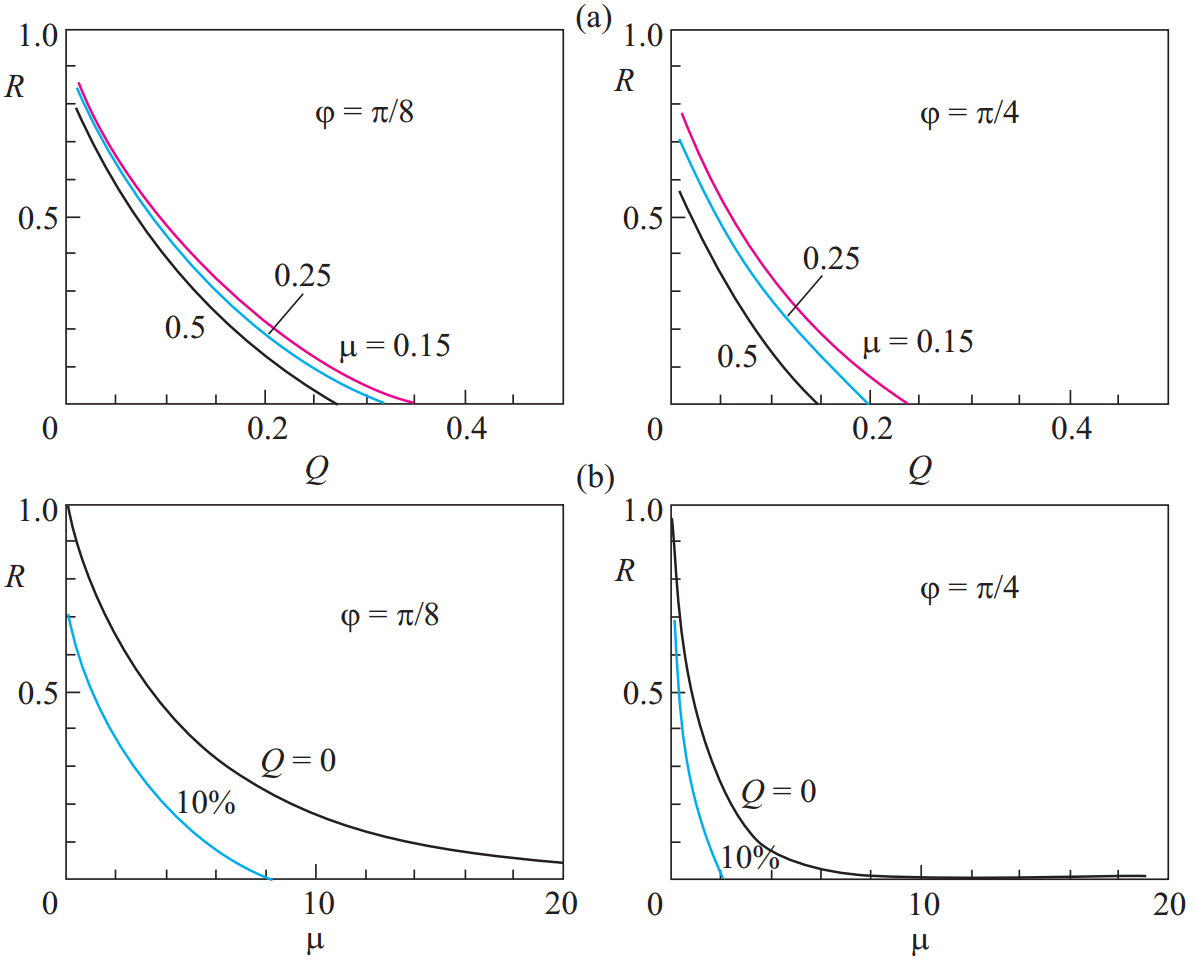
\includegraphics[width=0.9\linewidth]{key_rate}}
  \caption{Зависимость длины секретного ключа $R$ от наблюдаемой ошибки (а) и среднего числа фотонов (b)}
  \label{fig:key_rate}
  \end{figure}
